%%%%%%%%%%%%%%%%%%%%%%%%%%%%%%%%%%%%%%%%%
% University/School Laboratory Report
% LaTeX Template
% Version 3.1 (25/3/14)
%
% This template has been downloaded from:
% http://www.LaTeXTemplates.com
%
% Original author:
% Linux and Unix Users Group at Virginia Tech Wiki 
% (https://vtluug.org/wiki/Example_LaTeX_chem_lab_report)
%
% License:
% CC BY-NC-SA 3.0 (http://creativecommons.org/licenses/by-nc-sa/3.0/)
%
%%%%%%%%%%%%%%%%%%%%%%%%%%%%%%%%%%%%%%%%%

%----------------------------------------------------------------------------------------
%	PACKAGES AND DOCUMENT CONFIGURATIONS
%----------------------------------------------------------------------------------------

\documentclass{article}

\let\Item\item
\newcommand\SpecialItem{\renewcommand\item[1][]{\Item[\textbullet~\bfseries##1]}}
\renewcommand\enddescription{\endlist\global\let\item\Item}

\usepackage[utf8]{inputenc}

% Default fixed font does not support bold face
\DeclareFixedFont{\ttb}{T1}{txtt}{bx}{n}{12} % for bold
\DeclareFixedFont{\ttm}{T1}{txtt}{m}{n}{12}  % for normal

% Custom colors
\usepackage{color}
\definecolor{deepblue}{rgb}{0,0,0.5}
\definecolor{deepred}{rgb}{0.6,0,0}
\definecolor{deepgreen}{rgb}{0,0.5,0}

\usepackage[procnames]{listings}
\usepackage{color}

\definecolor{keywords}{RGB}{255,0,90}
\definecolor{comments}{RGB}{0,0,113}
\definecolor{red}{RGB}{160,0,0}
\definecolor{green}{RGB}{0,150,0}

\lstset{language=Python, 
	basicstyle=\ttfamily\small, 
	keywordstyle=\color{keywords},
	commentstyle=\color{comments},
	stringstyle=\color{red},
	showstringspaces=false,
	identifierstyle=\color{green},
	tabsize=4,
	procnamekeys={def,class}}

\usepackage[version=3]{mhchem} % Package for chemical equation typesetting
\usepackage{siunitx} % Provides the \SI{}{} and \si{} command for typesetting SI units
\usepackage{graphicx} % Required for the inclusion of images
%\usepackage{natbib} % Required to change bibliography style to APA
\usepackage{amsmath} % Required for some math elements 
\usepackage{diagbox}
\setlength\parindent{0pt} % Removes all indentation from paragraphs

\renewcommand{\labelenumi}{\alph{enumi}.} % Make numbering in the enumerate environment by letter rather than number (e.g. section 6)

\usepackage{tikz}
\def\checkmark{\tikz\fill[scale=0.4](0,.35) -- (.25,0) -- (1,.7) -- (.25,.15) -- cycle;} 

%\usepackage{times} % Uncomment to use the Times New Roman font

%----------------------------------------------------------------------------------------
%	DOCUMENT INFORMATION
%----------------------------------------------------------------------------------------

\title{ANLP Assignment 2} % Title

\author{
	Ida \textsc{Szubert}\\
	\texttt{s0907677}
	\and
	Yue \textsc{Yu}\\
	\texttt{s1563228}
}

\date{\today} % Date for the report

\begin{document}
%----------------------------------------------------------------------------------------
%	QUESTION 1
%----------------------------------------------------------------------------------------
\section{Tokenization}

Tokenizing a sentence by identifying strings which match

\begin{center}
\begin{tabular}{l r}
	{[}a-zA-Z{]}+&tokens consisting of any number of letters\\
	'[a-z]+&tokens consisting of ' proceeding any number of letters\\
	{[},.?;:()-{]}&tokens consisting of single punctuation marks\\
\end{tabular}
\end{center}
would be sufficient to account for the most common English uses of punctuation symbols, including recognizing as separate tokens possesive \emph{'s} and contractions such as \emph{'d, 't, 're}.  However, there is a number of problematic cases:

\begin{itemize}
	\item
	lone apostrophes as possessive suffix on nominals ending in s (such as \emph{flowers' pollen} meaning pollen of many flowers);
	\item
	ellipsis of the centuries part of a year (such as \emph{the '70s, in the '98});
	\item
	informal contractions (such as \emph{about $\rightarrow$ 'bout, unless $\rightarrow$  ’less, because $\rightarrow$  'cause, and $\rightarrow$ 'n'});
	\item
	surnames and lexical items with apostrophes (such as \emph{'o clock, O'Brian, M'Gregor});
\end{itemize}
The tokenize function changes the lone-apostrophes possessive into \emph{'s} so that a word can be tokenized into its main lexical part and the possessive suffix. It also recognizes contracted dates. The other two problems, being largely lexical, remain unsolved.

\begin{lstlisting}
def tokenise(tokenstring):
'''Split a string into a list of tokens, treating punctuation as
separate tokens, and splitting contractions into their parts.
So for example "I'm leaving." --> ["I","'m","leaving","."]'''
	# normalize possessive ' to possessive 's
	normalized_1 = re.sub(r"s'\b", "s's ", tokenstring)
	# if ' is followed by more that 2 digits, it's not a year
	# split into ' and digit string
	normalized_2 = re.sub(r"'(\d{3})", r"' \1", normalized_1)
	# find all alphanumeric strings, 'digit-digit strings, 's/'d/'m etc. strings
	# and single punctuation marks
	return re.findall(r"[a-zA-Z\d]+|'\d\d\b|'[a-z]*|[,.?;:()-]", normalized_2)
\end{lstlisting}
%----------------------------------------------------------------------------------------
%	QUESTION 2
%----------------------------------------------------------------------------------------
\section{Parse trees}
\begin{figure}[h!]
	\centering
	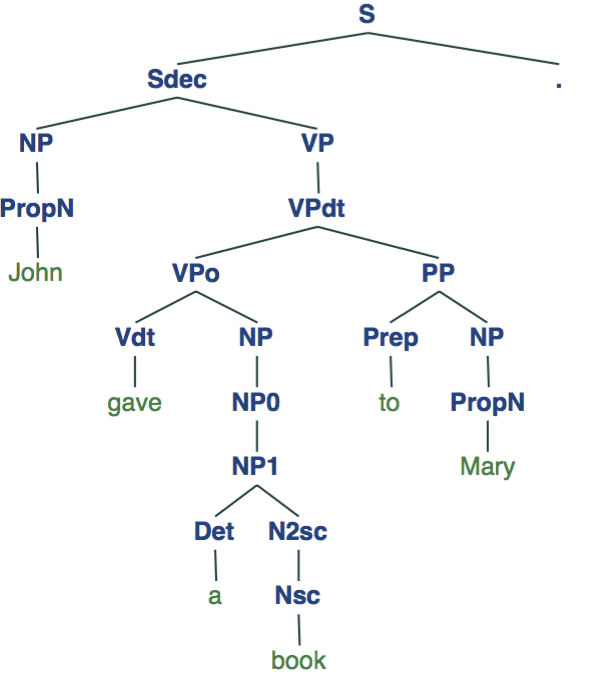
\includegraphics[width=0.4\linewidth]{../s1}
	\caption{\emph{John gave a book to Mary.}}
	\label{fig:s1}
\end{figure}
\begin{figure}[h!]
	\centering
	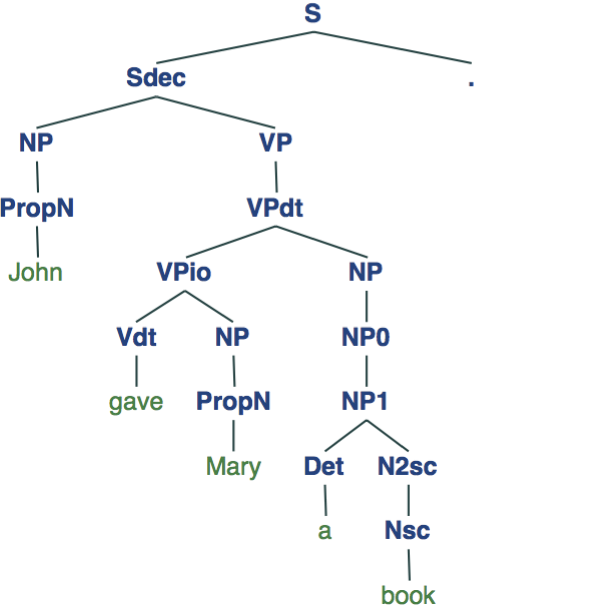
\includegraphics[width=0.4\linewidth]{../s2}
	\caption{\emph{John gave Mary a book.}}
	\label{fig:s2}
\end{figure}
\begin{figure}[h!]
	\centering
	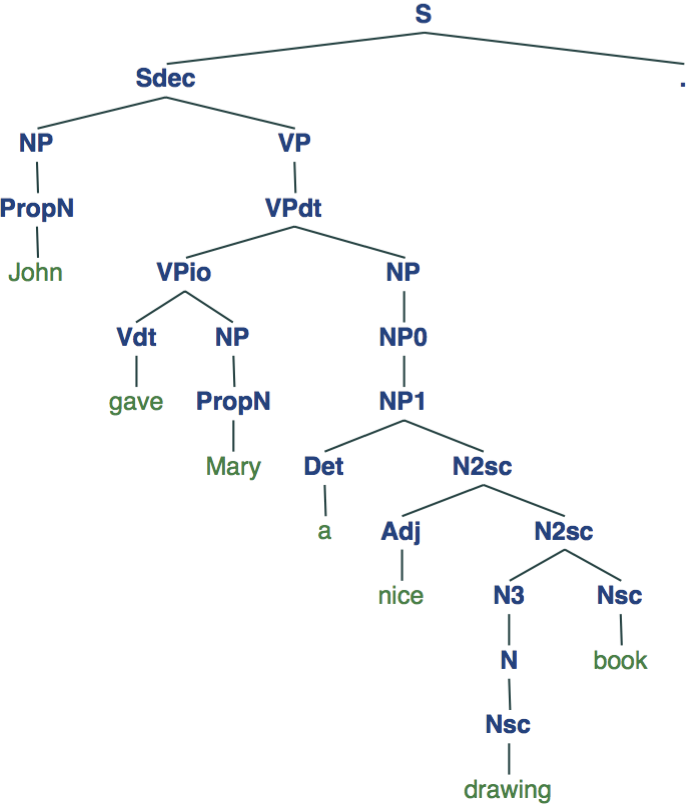
\includegraphics[width=0.4\linewidth]{../s3}
	\caption{\emph{John gave Mary a nice drawing book.}}
	\label{fig:s3}
\end{figure}
\begin{figure}[h!]
	\centering
	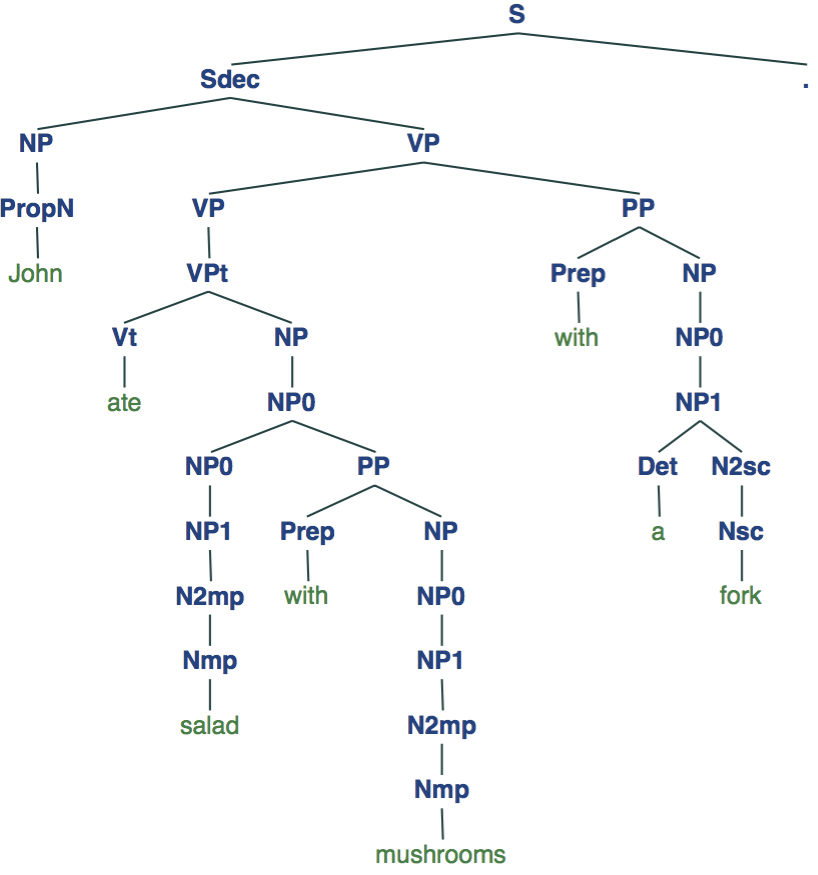
\includegraphics[width=0.4\linewidth]{../s4}
	\caption{\emph{John ate salad with mushrooms with a fork.}}
	\label{fig:s4}
\end{figure}
\begin{figure}[h!]
	\centering
	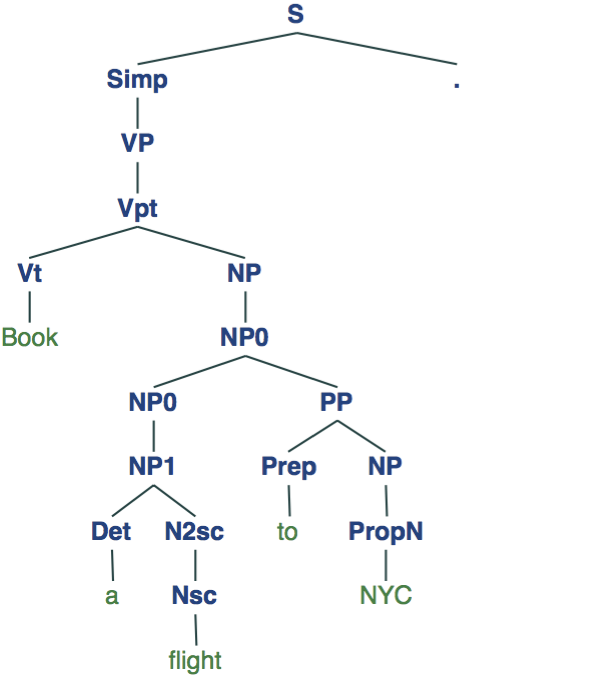
\includegraphics[width=0.4\linewidth]{../s5}
	\caption{\emph{Book a flight to NYC.}}
	\label{fig:s5}
\end{figure}
\begin{figure}[h!]
	\centering
	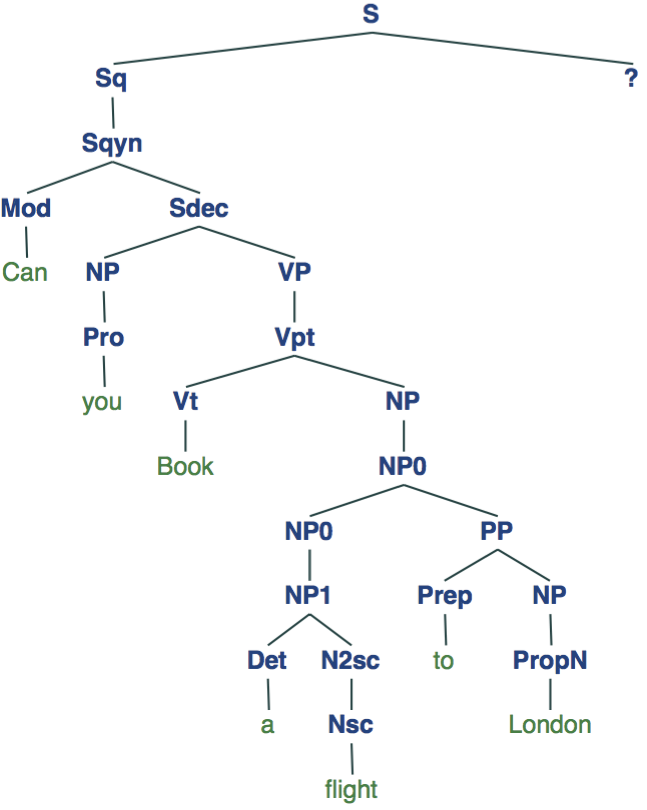
\includegraphics[width=0.4\linewidth]{../s6}
	\caption{\emph{Can you book a flight to London?}}
	\label{fig:s6}
\end{figure}
\begin{figure}[h!]
	\centering
	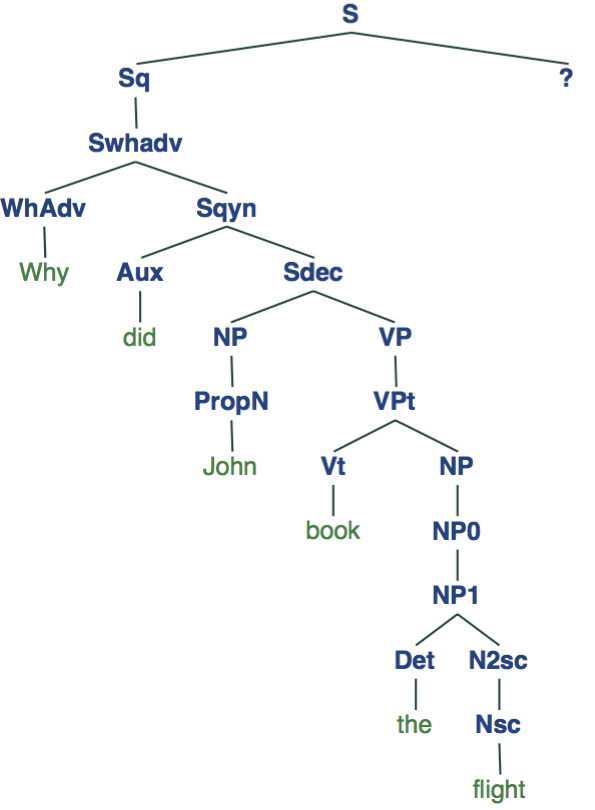
\includegraphics[width=0.4\linewidth]{../s7}
	\caption{\emph{Why did John book a the flight?}}
	\label{fig:s7}
\end{figure}
\begin{figure}[h!]
	\centering
	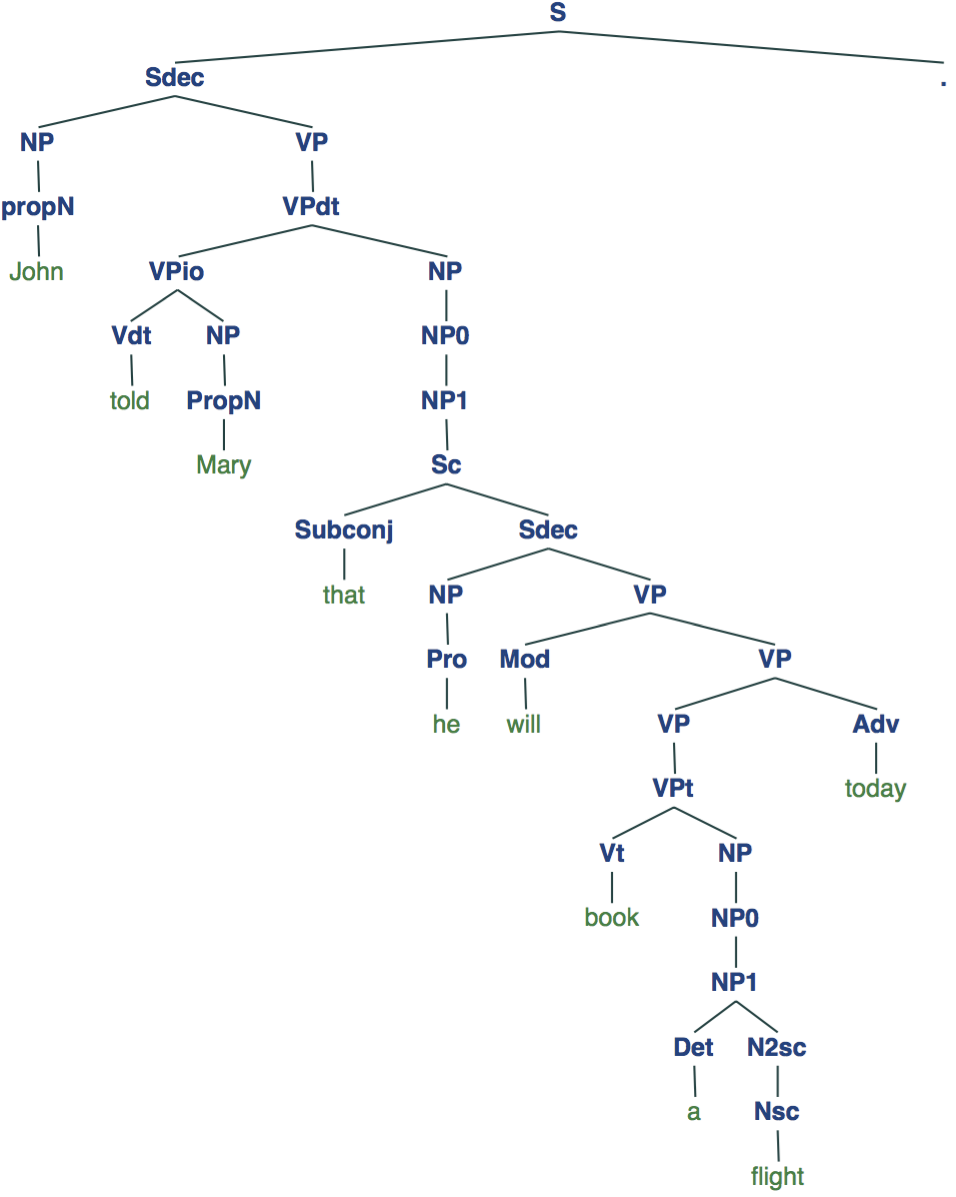
\includegraphics[width=0.4\linewidth]{../s8}
	\caption{\emph{John told Mary that he will book a flight today.}}
	\label{fig:s8}
\end{figure}

%----------------------------------------------------------------------------------------
%	QUESTION 3
%----------------------------------------------------------------------------------------
\section{Remarks on the grammar}

\begin{description}
	\subsection{Design of the grammar rules}
	\begin{enumerate}
		\item
		\textbf{Redundancy of rules in the verbal domain}
		
		There is a redundancy in the treatment of ditransitive verb phrases. \emph{VPo} an \emph{VPio} are two nodes which expand in the exact same way:
		\begin{center}
			
			\emph{VPo $\rightarrow$ Vdt NP} and \emph{VPio $\rightarrow$ Vdt NP}.
			
		\end{center}
		and therefore there is no difference between them within the grammar. From a linguistic point of view this separation might have a motivation. The ditransitive verb and its direct object are represented by \emph{Po}, while \emph{VPio} is a unit consisting of a ditransitive verb and its indirect object. As valid linguistic distinction as it might be, it does not need to be included in simple grammar like the one discussed here. In particular, no use is made of the distinction between that would limit overgenration. If that was the case, then having both non-terminals would be a valid design choice. For instance, one might consider putting some restrictions on what kinds of NP can be direct or indirect objects.
		The needless distinction between \emph{VPo} an \emph{VPio} propagates up to the topmost VP expansion rules. As a result, there are more VP-related rules than necessary. The grammar contains
		\begin{center}
			
			\emph{VP $\rightarrow$ VPi $\vert$ VPt $\vert$ VPdt $\vert$ Mod VP $\vert$ VP Adv $\vert$ VP PP}
			
			\emph{VPdt $\rightarrow$ VPo PP}
			
			\emph{VPdt $\rightarrow$ VPio NP}
			
			\emph{VPo $\rightarrow$ Vdt NP}
			
			\emph{VPio $\rightarrow$ Vdt NP}
			
		\end{center}
		but it could have contained as little as three rules instead:
		
		\begin{center}
			
			\emph{VP $\rightarrow$ VPi $\vert$ VPt $\vert$ VPdt $\vert$ Mod VP $\vert$ VP Adv $\vert$ VP PP}
			
			\emph{VPdt $\rightarrow$ VPd NP $\vert$ VPd PP}
			
			\emph{VPd $\rightarrow$ Vdt NP}
			
		\end{center}
		
		
		\item
		\textbf{Redundancy of rules in the nominal domain}
		
		Redundancy can be also observed among the nominal rules. The \emph{NP\textsubscript{0}} non-terminal node seems redundant. It's purpose is to allow for recursive generation of prepositional phrases following a noun phrase. This can be achieved by accounting for this kind of recursion within one of the existing NP rules. We could propose two sets of rules to replace the following:
		\begin{center}
			NP $\rightarrow$ PropN $\vert$  Pro $\vert$  NP\textsubscript{0}
			
			NP\textsubscript{0} $\rightarrow$ NP\textsubscript{1} $\vert$  NP\textsubscript{0} PP
			
			NP\textsubscript{1} $\rightarrow$ Det N2sc $\vert$  N2mp $\vert$  Sc
			
		\end{center}
		The first replacement option moves recursive \emph{PP} addition into an \emph{NP} expansion rule:
		\begin{center}
			
			NP $\rightarrow$ PropN $\vert$ Pro $\vert$ NP\textsubscript{1} $\vert$ NP PP
			
			NP\textsubscript{1} $\rightarrow$ Det N2sc $\vert$  N2mp $\vert$  Sc
			
		\end{center}
		Such rearrangement has the advantage of allowing for not only common nouns, but also proper names and pronouns to be modified by \emph{PPs}. This could be desirable in a more comprehensive grammar, but additional restrictions would be required, e.g. to account for pronouns generally not taking \emph{PP} complements.
		The second option moves the recursion into an \emph{NP\textsubscript{1}} expansion:
		\begin{center}
			
			NP $\rightarrow$ PropN $\vert$  Pro $\vert$  NP\textsubscript{1}
			
			NP\textsubscript{1} $\rightarrow$ Det N2sc $\vert$ N2mp $\vert$ Sc $\vert$ NP\textsubscript{1} PP
			
			
		\end{center}
		
		It is more conservative in that with these rules in replacing the originals, the grammar would generate the same strings, i.e. the grammars with and without replacement would be weakly equivalent [TODO citation].
		The \emph{NP\textsubscript{0}} node expands to an \emph{NP\textsubscript{1}} followed by an arbitrary number of \emph{PPs}. The same effect will be achieved by recursively expanding \emph{NP\textsubscript{1}}  into an \emph{NP\textsubscript{1}} and  \emph{PP}, with the benefit of reducing the number of non-terminals.
		
		One might argue that linguistic justification of the existence of the \emph{NP\textsubscript{0}} can be found in its correspondence with N' node in X-bar syntax. Both are projections above N and below full NP, and allow for adding in principle an unlimited number of modifiers to the head N-complement unit[TODO citation]. However, the recursive expansion of the \emph{NP\textsubscript{0}} node implies that PPs to the right of head N are adjuncts rather than complements of that N, which is not true. [TODO citation]. The similarity between \emph{NP\textsubscript{0}} and N' is superficial and can be rejected as motivation for including the former in the grammar. 
		
		\item
		\textbf{Dobtfull usefulness of the \textit{Sq} node}
		
		The \emph{Sq} node serves no purpose other than to reflect the conceptual relation between \emph{Sqyn} and \emph{Swhadv}, namely the fact both are non-terminals expanding into questions. This, however, represents only a superficial, if not mistaken, grammatical insight. In fact wh-questions and auxiliary-inversion questions are represented by very different structures (WH-phrases and Aux-phrases respectively[TODO citation]). If the motivation for including the \emph{Sq} node it linguistic, then the reasons seem insufficient.
		If, one the other hand, the node was included in the grammar to simplify the expansion of \emph{S}, then by analogy we should also include
		\begin{center}
			
			\emph{Sd $\rightarrow$ Sdec $\vert$ Simp}
			
		\end{center}an change the expansion of \emph{S} to
		\begin{center}
			
			\emph{S $\rightarrow$ Sd '.' $\vert$ Sq '?'}
			
		\end{center}
		
		\item
		\textbf{Lower case and capitalized versions of terminals.}
		
		It does not seem necessary to include lower case and capitalized versions of the same terminals. In the sample sentences we have seen \textit{Book, Can}, and \textit{Why} being capitalized to account for their sentence-initial positions. instead of duplicating lexical items, we could simply capitalize  the first word of a generated sentence and ignore sentence-initial capitalization during parsing.
		There would be no ill effects of such a change, since every generated sentence is, by definition, grammatical. Every word which happens to be initial in a sentence produced by the grammar is allowed to be there. The additional confirmation of this fact in form of the word's capitalised version being present in the grammar is unnecessary.
	\end{enumerate}
	\subsection{Overgeneration}
	\begin{enumerate}
		\item
		\textbf{Lack of subject-verb agreement}
		
		There’s distinction between single/count and plural/mass nouns, but no corresponding distinction in the verbal domain. The problem is somewhat masked by the fact that most of the included verbs are in past tense, where in English there are no subject-verb agreement phenomena. Nevertheless, we can see that the grammar would accept  \emph{*the fork book a flight.}, a sentence which ignores verb conjugation requirements.
		
		\item
		\textbf{Treating VP as full sentences}
		
		The rules:
		\begin{center}
			
			S $\rightarrow$ Simp ‘.’
			
			Simp $\rightarrow$ VP
			
		\end{center}
		imply that any \emph{VP} can be a grammatical sentence on its own. This, however, is true only of \emph{VP} in imperative mood. The grammar, however, allows for treating any \emph{VP}, e.g. \emph{*ate today}, as a full sentence. Solving this problem is not possible without substantially expanding the grammar. We would have to distinguish between infinitival and inflected forms of verbs, and extend the set of possible expansions of \emph{VP} accordingly. We could then state that \emph{Simp} subcategories for \emph{VPs} whose head is an infinitival form of a verb. Therefore, we would need the following rules:
		\begin{center}
			
			$Vt_inf$ $\rightarrow$ ‘Book’ $\vert$ ‘Tell’ $\vert$ …
			
			$VPi_inf$ $\rightarrow$ ‘Eat' $\vert$ …
			
			$VPt_inf$ $\rightarrow$ $Vt_inf$ NP $\vert$ $VPt_inf$ Adv $\vert$ $VPt_inf$ PP
			
			VP $\rightarrow$ $VPt_inf$
			
			Simp $\rightarrow$ $VPt_inf$ $\vert$ $VPi_inf$
			
		\end{center}
		Even then, additional restrictions would be needed to account for characteristics of the imperative mood, e.g. the fact that the second person pronoun needs to be in its reflexive form when used as a direct object of the matrix verb [TODO citation] . Otherwise the grammar would generate sentences such as \emph{*Book you a flight to London.} instead of grammatical \emph{*Book yourself a flight to London.}
		
		\item
		\textbf{Case agreement}
		
		The grammar does not account for case subcategorisation requirements of verbs. The only corner of the modern English syntax which still exhibits case phenomena is the pronoun system[TODO citation], however the grammar does not include a \emph{ProNom} and a \emph{ProAcc} pre-terminals. Having no distinction between nominative and accusative forms leads to admitting non-grammatical sentences, e.g.\emph{*Mary gave \textbf{he} a nice salad.} instead of \emph{Mary gave \textbf{him} a nice salad.}
		
		\item
		\textbf{Verb and noun subcategorization for pronouns}
		
		Verbs an nouns tend to co-occur with particular pronouns more often than with others. However, the grammar does not account for this preference. For instance, one can \emph{eat with a fork}, \emph{eat with Mary}, or have a \emph{flight to London}, but the grammar also allows for having a \emph{*salad to fork} and booking a \emph{*flight with NYC.}
		
		\item
		\textbf{Multiple modals}
		
		The grammar allows for an unlimited number of modals to proceed a \emph{VP}. This can lead to generating sentences such as \emph{*Can will can can John book a flight?}. However, English limits the acceptable number (up to 4, depending on dialetct), orderings (evidential, epistemic, deontic), and identity (\emph{might} or \emph{may} being the most commonly first in the sequence (Di Paolo 1989)) of verbs in multiple modal constructions. In order to capture these restrictions we would need a whole series of serially connected expansion rules, each introducing one modal of a certain type.
	\end{enumerate}
\end{description}
%----------------------------------------------------------------------------------------
%	QUESTION 4
%----------------------------------------------------------------------------------------

\section{Comments for CKY.buildIndices}

\begin{lstlisting}
def buildIndices(self,productions):
	""" Creates dictionaries for storing the production rules.
	    In each dictionary, the rhs of a rule is the key and and
	    a list of all lhs which expand as the rhs is the value."""
	
	# create dictionaries for unary and binary rules
	self.unary=defaultdict(list)
	self.binary=defaultdict(list)
	
	for production in productions:
		# separate its right hand-side from its left hand-side
		rhs=production.rhs()
		lhs=production.lhs()
		# the assumption about the rules is that rhs is non-empty
		# and rhs has no more than 2 non-terminals
		assert(len(rhs)>0 and len(rhs)<=2)
		# if the rule is unary, 
		# add it's lhs to the unary dictionary under rhs key
		if len(rhs)==1:
			self.unary[rhs[0]].append(lhs)
		# if the rule is binary, 
		# add it's lhs to the binary dictionary under rhs key
		# because of the assertion we know that len(rhs)==2
		else:
			self.binary[rhs].append(lhs)
\end{lstlisting}

\hfill \break

%----------------------------------------------------------------------------------------
%	QUESTION 5
%----------------------------------------------------------------------------------------

\section{Comments for CKY.unary\_fill \& Cell.unary\_update}
\begin{lstlisting}
def unary_fill(self):
	"""Determine the possible non-terminals that 
	   each terminal can result from. 
	   Fill the results in the middle diagonal and print"""
	
	for r in range(self.n-1):
		# the middle diagonal
		cell=self.matrix[r][r+1]
		# initialize the cell
		word=self.words[r]
		cell.addLabel(word)
		# recursively update the cell
		cell.unary_update(word,self.unary)
		# print out the possible non-terminals for each cell (terminal)
		if self.verbose:
			print "Unary branching rules at node (%s,%s):%s"%(r,r+1,cell.labels())
			
def unary_update(self,symbol,unaries):
	"""Update the cell labels by adding non-terminals 
	   which expand as the given symbol"""
	   
	# if the symbol is a right hand-side of a unary production rule
	if symbol in unaries:
		# add each of possible corresponding left hand-sides
		# to the cell's labels
		for parent in unaries[symbol]:
			# only add labels that is not in the cell already
			# to avoid the exponential cost of the recognition process
			if parent not in self._labels:
				self.addLabel(parent)
				# a recursive call is needed because in the grammar 
				# not all unary productions are terminal productions
				self.unary_update(parent,unaries)
\end{lstlisting}

\hfill \break
%----------------------------------------------------------------------------------------
%	QUESTION 6
%----------------------------------------------------------------------------------------

\section{Comments for CKY.parse \& CKY.maybe\_build}
\begin{lstlisting}
def maybe_build(self, start, mid, end):
	"""Search for the possible combinitions of 
	   the symbols in two given cells (one from each) 
	   to match the rhs of binary branching rules"""
	   
	if self.verbose:
		print "Binary branching rules for %s--%s--%s:"%(start,mid,end),
	
	cell=self.matrix[start][end]
	
	# search from the given cells
	for s1 in self.matrix[start][mid].labels():
		for s2 in self.matrix[mid][end].labels():
			# for a binary branching rule match
			if (s1,s2) in self.binary:
				# add all possible non-terminals
				# from the lhs of the rule
				for s in self.binary[(s1,s2)]:
					cell.addLabel(s)
					# add more possible non-terminals 
					# because, in the grammar, there are unary rules 
					# that can produce non-terminals
					cell.unary_update(s,self.unary)
					if self.verbose:
						print " %s -> %s %s"%(s, s1,s2),
	if self.verbose:
		print 

\end{lstlisting}
\hfill \break

*All the comments above are included in \textit{cky.py}

\hfill \break

%----------------------------------------------------------------------------------------
%	QUESTION 7
%----------------------------------------------------------------------------------------

\section{Ambiguity Analysis}

\subsection{"John gave a book to Mary."}

\textbf{Distinct Parse(s):} 3\\

\textbf{Ambiguity Source:} 3 different \textbf{VPs} found in (1,6) can pair up with the \textbf{NP} in (0,1) to form \textbf{Sdecl}. The \textbf{VPs} came from the following rules:

\begin{center}
	\textbf{\emph{VP $\rightarrow$ VP(1,4) PP(4,6)}\\
	\emph{VP $\rightarrow$ VPdt $\rightarrow$ VPo(1,4) PP(4,6)}\\
	\emph{VP $\rightarrow$ VPt $\rightarrow$ Vt(1,2) NP(2,6)}}
\end{center}

\textbf{Interpretation of ambiguity:}\\
{[}VP {[}VP John gave a book{]} {[}PP to Mary{]}{]}

In this parse, \emph{John gave a book} is a full VP, and \emph{to Mary} is an additional modifier. This an analysis would be correct for a sentence such as \emph{John read a book on the couch}, where \emph{the couch} is not an argument of the verb. In case of \emph{give} both the NP and the PP are arguments.

[VP [VPdt [VPo John gave a book] [PP to Mary]]]

This is the most appropriate parse, in which \emph{give} has a direct object, \emph{a book}, and an indirect one, \emph{Mary}. The only VP in this analysis is the one which correctly encompasses all of the participants of the event.

[VP [VPt [Vt John gave] [NP a book to Mary]]]

This analysis incorrectly treats \emph{to Mary} as forming as a modifier of \emph{a book}. This structure would correctly describe a sentence such as \emph{John ate pasta with tuna}, where the PP really modifies the noun, and the verb really is transitive.

\subsection{"John gave Mary a book."}

\textbf{Distinct Parse(s):} 1

\subsection{"John gave Mary a nice drawing book."}

\textbf{Distinct Parse(s):} 2\\

\textbf{Ambiguity Source:} 2 different \textbf{N2sc} found in (4,7) can pair up with the \textbf{Det} in (3,4) to form \textbf{NP1}. The \textbf{N2sc} came from the following rules:

\begin{center}
\emph{N2sc $\rightarrow$ Adj(4,5) N2sc(5,7)}\\
\textbf{\emph{N2sc(5,7) $\rightarrow$ N3(5,6) Nsc(6,7)}\\
\emph{N2sc(5,7) $\rightarrow$ Adj(5,6) N2sc(6,7)}}
\end{center}

\textbf{Interpretation of ambiguity:}\\
{[}N2sc {[}Adj drawing{]} {[}Nsc book{]}{]}

The grammar lists \emph{drawing} as an adjective, so the unit \emph{drawing book} can be analysed as a noun modified by an adjective, in the way \emph{fragile} is a modifier in \emph{fragile cup}.

{[}N2sc {[}N3 {[}N drawing{]}{]} {[}Nsc book{]}{]}

In this parse both \emph{drawing} and \emph{book} are treated as nouns, and N2sc represents a noun-noun compound, in the way \emph{tea cup} is a compound of two nouns. This seems to be a correct interpretation, given how popular such structures are in English, and that there is no evidence of \emph{drawing} being an adjective (e.g. there are no comparative forms \emph{*a drawinger book }).

\subsection{"John ate salad with mushrooms with a fork."}

\textbf{Distinct Parse(s):} 5\\

\textbf{Ambiguity Source:} 5 different \textbf{VP} found in (1,8) can pair up with the \textbf{NP} in (0,1) to form \textbf{Sdecl}. The \textbf{VP} came from the following rules:

\begin{center}
	\textbf{\emph{VP $\rightarrow$ VP(1,3) PP(3,8)}}\\
	
	\emph{VP $\rightarrow$ VP(1,5) PP(5,8)}
	
	\textbf{\emph{VP(1,5) $\rightarrow$ VP(1,3) PP(3,5)}\\
	\emph{VP(1,5) $\rightarrow$ VPt $\rightarrow$ Vt(1,2) NP(2,5)}}\\

	\emph{VP $\rightarrow$ VPt $\rightarrow$ Vt(1,2) NP(2,8) $\rightarrow$ NP0}\\
	\textbf{\emph{NP0 $\rightarrow$ NP0(2,3) PP(3,8)}\\
	\emph{NP0 $\rightarrow$ NP0(2,5) PP(5,8)}}
\end{center}

\textbf{Interpretation of ambiguity:}\\

\subsection{"Book a flight to NYC."}

\textbf{Distinct Parse(s):} 2\\

\textbf{Ambiguity Source:} 2 different \textbf{Simp} found in (0,5) can pair up with the \textbf{'.'} in (5,6) to form \textbf{S}. The \textbf{Simp} came from the following rules:

\begin{center}
	\emph{Simp $\rightarrow$ VP}\\
	\textbf{\emph{VP $\rightarrow$ VP(0,3) PP(3,5)}\\
	\emph{VP $\rightarrow$ VPt $\rightarrow$ Vt(0,1) NP(1,5)}}
\end{center}

\textbf{Interpretation of ambiguity:}\\

\subsection{"Can you book a flight to London?"}

\textbf{Distinct Parse(s):} 2\\

\textbf{Ambiguity Source:} 2 different \textbf{Sq} found in (0,7) can pair up with the \textbf{'?'} in (7,8) to form \textbf{S}. The \textbf{Sq} came from the following rules:

\begin{center}
	\emph{Sq $\rightarrow$ Sqyn $\rightarrow$ Mod(0,1) Sdecl(1,7)}\\
	\emph{Sdecl(1,7) $\rightarrow$ NP(1,2) VP(2,7)}\\
	\textbf{\emph{VP(2,7) $\rightarrow$ VP(2,5) PP(5,7)}\\
	\emph{VP(2,7) $\rightarrow$ VPt $\rightarrow$ Vt(2,3) NP(3,7)}}
\end{center}

\textbf{Interpretation of ambiguity:}\\

\subsection{"Why did John book the flight?"}

\textbf{Distinct Parse(s):} 1

\subsection{"John told Mary that he will book a flight today."}

\textbf{Distinct Parse(s):} 3\\

\textbf{Ambiguity Source:} 3 different \textbf{Sdecl} found in (0,10) can pair up with the \textbf{'.'} in (10,11) to form \textbf{S}. The \textbf{Sdecl} came from the following rules:

\begin{center}
	\emph{Sdecl $\rightarrow$ NP(0,1) VP(1,10)}\\
	\textbf{\emph{VP(1,10) $\rightarrow$ VP(1,9) Adv(9,10)}}\\
	\emph{VP(1,10) $\rightarrow$ VPdt $\rightarrow$ VPio(1,3) NP(3,10)}\\
	
	\emph{NP(3,10) $\rightarrow$ NP0 $\rightarrow$ NP1 $\rightarrow$ Sc $\rightarrow$ Subconj(3,4) Sdecl(4,10)}\\
	\emph{Sdecl(4,10) $\rightarrow$ NP(4,5) VP(5,10)}\\
	\textbf{\emph{VP(5,10) $\rightarrow$ Mod(5,6) VP(6,10)}\\
	\emph{VP(5,10) $\rightarrow$ VP(5,9) Adv(9,10)}}
\end{center}

\textbf{Interpretation of ambiguity:}\\


%----------------------------------------------------------------------------------------
%	QUESTION 8
%----------------------------------------------------------------------------------------

\section{Generating a parse tree}

\subsection{CKY parsing}

Up to now, the program is a CKY recognizer that can only determine whether a string belongs to the language generated by the given grammar. In order to extend it into a CKY parser that can construct a parse tree, back-pointers, which records the one or more ways in which a constituent spanning (i,j) can be made from constituents spanning (i,k) and (k,j), will be attached to each label in the table cells. Therefore, after successful parsing, we can traceback from the Start Symbols (S) in the top-right-hand corner of the matrix to every terminals from the string. The final result is then a shared-forest of possible parse trees, where common tree parts are factored between the various parses \cite{lang1994recognition}.

\subsection{Design and implementation}
First, a Label class was defined to describe the labels in each cell which was represented by String. Benefited from the flexible data structure in Python, this class can be initialized with at most 4 parameters, as shown below.\\

List of parameters:

\SpecialItem
\begin{description}
	\item[symbol] the represented label (required)
	\item[start] row number of the cell (optional)
	\item[end] column number of the cell (optional)
	\item[rhs] list of right-hand-sides of the production rules which generate the target symbol; mid value is also included in the list, which refers to the source cells from which the constituents of right-hand-sides came (optional)
\end{description}

The Label class can take different number of parameters depending on where the label came from, such as the left-hand-sides of rules and words from the input string. For instance, if a symbol was added according to a unary rule, the row number and column number will be the same as its parent label which we already knew. For the labels of words, which will be the leaf nodes of a parse tree, the value of right-hand-side will be omitted (not available).

\begin{table}[h]
	\centering
	\begin{tabular}{|c|c|c|c|}\hline
		\diagbox[width=12em]{\\Parameter}{\\Source Type}&
		binary rule & \shortstack{unary rule} & word \\ \hline
		symbol & \checkmark            & \checkmark        & \checkmark    \\ \hline
		start  & \checkmark            & ~        & ~    \\ \hline
		end    & \checkmark            & ~        & ~    \\ \hline
		rhs    & \checkmark            & \checkmark        & ~    \\ \hline
	\end{tabular}
	\caption{Parameter Structure for Different Labels}\label{tab:flexible}
\end{table}

Moreover, a number of the existing CKY and Cell methods were edited to construct/exploit this richer label structure. Three utility functions for listing, searching and updating label list are also provided.\\

After that, the backtrack algorithm was implemented in two functions:

\SpecialItem
\begin{description}
	\item[update\_trees] to update all the possible subtrees of the give label in a cell (In this implementation, the function will be ended after the first subtree was returned)
	\item[update\_children] to construct NLTK tree nodes according to given rules
\end{description}

\textit{update\_trees} and \textit{update\_children} will call each other recursively to generate the whole parse tree.

\subsection{Summary}
To generate the first parse tree, we only need to pass the Start Symbols (S) in the top-right-hand corner of the matrix to \textit{update\_trees} method and it will return the result after the first parse tree was found. However, in order to return all the possible parse trees, the Start Symbols (S) in the top-right-hand corner of the matrix should be treated differently from other labels and \textit{update\_trees} method should return a list of possible subtrees to construct all the ambiguous result. The detail of generating all parse trees will not be discussed in this report.


%----------------------------------------------------------------------------------------
%	BIBLIOGRAPHY
%----------------------------------------------------------------------------------------

\bibliographystyle{ieeetr}

\bibliography{sample}

%----------------------------------------------------------------------------------------


\end{document}